\chapter{Problemanalyse}
\textit{I dette kapitel analyses problemstillinger, som opstår i forbindelse med lægemiddelskift. Disse problemstillinger vil sammenfattes i en opsummering og afsluttes med en problemformulering, der fremadrettet danner  grundlaget for rapporten.}

\section{Udbud og indkøb af lægemidler}
Siden år 2007 har Amgros, Regionens lægemiddelorganisation, årligt sendt lægemidler i udbud med henblik på at mindske udgifterne til sygehusmedicin.~\citep{Sygehusapoteket2017, Amgros2017} I år 2017 sparede Amgros samlet regionerne for 3,1 milliarder kroner.~\citep{Amgros2015} Udbud forekommer på lægemidler, hvor der findes mere end én leverandør~\citep{Amgros2015}. Amgros bringer på denne måde lægemidlerne i konkurrence og bestræber sig på at indkøbe lægemidler af høj kvalitet til bedst mulige priser til de offentlige danske hospitaler~\citep{Amgros2015}.

En gang årligt fra start september til midt november sendes størstedelen af lægemidler i Anatomisk Terapeutisk Kemisk (ATC) gruppe i udbud, hvor udbud på ATC-grupper som indgår i Medicinrådets behandlingsvejledninger sker løbende hen over året~\citep{Sygehusapoteket2017}. Forinden et udbud foretages defineres antallet af vindere samt, hvorvidt udbuddet skal vurderes ud fra laveste pris eller være mest økonomisk fordelagtig~\citep{Amgros2018a}, hvilket er beskrevet i Appendiks \ref{cha:AppB}. Ved mest økonomisk fordelagtig vægtes prisen mod andre kriterier som er opstillet ud fra et juridisk grundlag og kan f.eks. omfatte lægemidlets emballage, håndtering, administration eller patientsikkerhedsmæssige aspekter~\citep{Amgros2018a}.

Inden et lægemiddel anvendes som standardbehandling foretages analyser og vurderinger af Amgros og Medicnrådet, som er yderligere beskrevet i Appendiks \ref{cha:AppA}. På baggrund af disse analyser og vurderinger foretages et kontraktskift mellem Amgros og den kommende leverandør af lægemidlet.

\section{Levering af lægemidler}
Sygehusapoteker står for produktion og levering af lægemidler til hospitaler og institutioner. Apoteket har et samarbejde med Amgros ...

\section{Substitution af lægemidler}
Kontraktskift medfører substitution af lægemidler, hvor et lægemiddel udskiftes til et andet lægemiddel. Der findes to typer af substitution herunder analoge lægemidler og generiske lægemidler. Analoge lægemidler indeholder forskelligt aktive stof, har omtrent samme effekt og bivirkninger. Denne form for substitution kræver ændringer i  recept, hvorfor denne skal ordineres af en læge. Generiske lægemidler indeholder samme aktive stof, hvorved lægemidlerne fungerer som hinandens synonyme. Denne type af substitution kræver modsat analog substitution ikke ændringer af recept og kan derfor ordineres af en sygeplejerske. 

** Lægemiddelstyrelsen bestemmer om generisk substitution af lægemidler ***


\section{Problemstillinger ved substitution}
Substitution af lægemidler kan medføre patientsikkerhedsmæssige konsekvenser~\citep{DanskSelskabforPatientsikkerhed2009}. Et norsk studie har undersøgt konsekvenserne ved generisk substitution~\citep{Hakonsen2010}. Interview med 100 sygeplejersker påviste at der opstod fejlmedicinering ved generiske lægemidler~\citep{Hakonsen2010}. Ud af disse følte 92~\% af sygeplejerskerne at generiske lægemidler var tidskrævende og 91~\% at risikoen for fejl øges ved dispensering, hvoraf 42~\% havde oplevet fejl som følge af generisk substitution~\citep{Hakonsen2010}. Dokumeneterede medicineringsfejl ved generisk substitution fremgår af Figur \ref{fig:GeneriskSubstitution}.

\begin{figure}[H]\centering	\includegraphics[width=1\textwidth]{billeder/GenSub.png} 
	\caption{Medicineringsfejl ved generisk substitution rapporteret (n=100)~\citep{Hakonsen2010}.}
	\label{fig:GeneriskSubstitution}  
\end{figure}

Det fremgår af Figur \ref{fig:GeneriskSubstitution} at størstedelen af fejlmedicinering ved generisk substitution skyldes forkert lægemiddel, hvor en mindre del skyldes forkert formulering og i sjældnere tilfælde forkert dosis, administrationsvej og udeladelse af dosis. Forkert lægemiddel forstås som at et andet lægemiddel end der oprindeligt er dispenseret. Formulering beskriver lægemidlets fysiske form som f.eks. tabelletform, dosis beskriver mængden af lægemidlet og administrationsvej beskriver hvordan leveringen eller indgiften af et lægemiddel tages f.eks. via munden, peroralt.

Det norske studie undersøgte ligeledes årsagerne til medicineringsfejl, hvilket er rapporteret af 42 sygeplejersker~\citep{Hakonsen2010} og fremgår af Figur \ref{fig:GeneriskSubstitution1}.

\begin{figure}[H]\centering	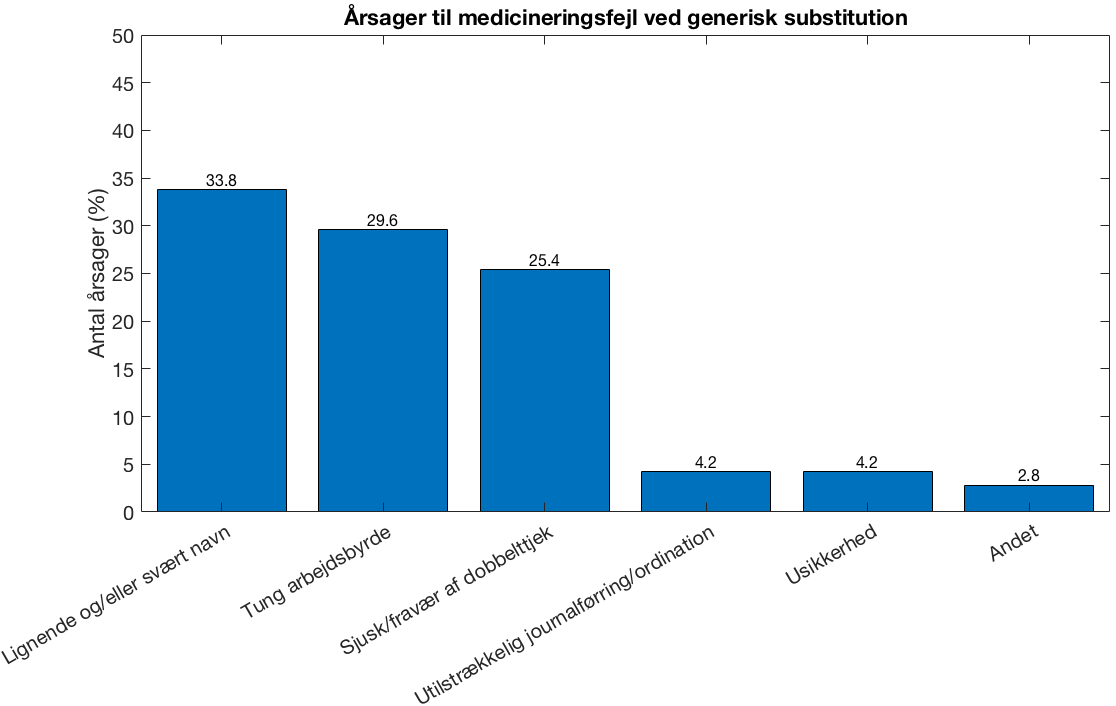
\includegraphics[width=1\textwidth]{billeder/GenSub1.png} 
	\caption{Årsager til medicineringsfejl ved generisk substitution (n=42)~\citep{Hakonsen2010}.}	\label{fig:GeneriskSubstitution1}  
\end{figure}

Af Figur \ref{fig:GeneriskSubstitution1} fremgår det at størstedelen af årsagerne til medicineringsfejl ved generisk substitution skyldes lignende og/eller vanskeligt lægemiddelnavn, kraftig arbejdsbyrde og sjusk eller fravær af dobbelttjek. En mindre del skyldes utilstrækkeligt journalførring og/eller ordination, usikkerhed eller andet. 

I flere lande, inklusiv Danmark, opstår forkert lægemiddel ofte i forbindelse med forvirring ved forveksling af navn eller emballage~\citep{DanskSelskabforPatientsikkerhed2009}, hvilket afspejles i det norske studie. Et eksempel på forveksling af navn er panodil, som er et smertestillende, og plendil, som anvendes til behandling af forhøjet blodtryk. Disse fejl kan forekomme som følge af lægemidler med, uden eller forskellige suffix/præfix, som f.eks. Efexor kontra Efexor Depot, Levemir penfill kontra Levemir flexpen, hvilket kan give anledning til dispensering af et forkert lægemiddel.~\citep{DanskSelskabforPatientsikkerhed2009}

Nogle af sygeplejersker i det norske studie mente at forvirringen over at finde det korrekte substitution medvirkede til at dosering og formulation var skyld i medicineringsfejl~\citep{Hakonsen2010}. Forveksling af lægemiddelnavne har i sjældnere tilfælde haft konsekvenser som har medført forlænget indlæggelse, forværret sygdom eller dødsfald.~\citep{DanskSelskabforPatientsikkerhed2009}

I takt med at hospitaletsmedicin opgørelse gennemgår ændringer jævnligt og antallet af generiske substitutioner stiger medvirker dette til at arbejdsbyrden er steget~\citep{Hakonsen2010}. Til trods for at sygeplejerskernes arbejde er blevet mere kompleks og krævende har de kun modtaget en begrænset oplæring inden for området.~\citep{Hakonsen2010}

I forhold til sjusk og fravær af dobbelttjek blev det i det norske studie rapporteret af 27~\% sygeplejersker at det var kutyme at en anden sygeplejerske dobbelttjekkede medicinen før den blev givet til patienten~\citep{Hakonsen2010}. Yderligere angav 48~\% at dobbelttjekket kun skete i de tilfælde hvor de var usikre over situation.~\citep{Hakonsen2010} På trods af at dette er et norsk studie forventes det at lignende problemstillinger kan relateres til Danmark.

Generelt set er medicinering den hyppigste årsag til rapportering af utilsigtede hændelser i år 2013~\citep{Patientombuddet2013}. Antallet af rapportering er i Region Nordjylland steget med over 36~\% fra år 2012 til 2012. Ud af 824 rapporterede utilsigtede hændelser i år 2014 omhandlede 97\% medicinering, 86\% administration af medicin og 41\% disponering~\citep{Jensen2014}, hvor mere end en rapporterede hændelse kan omhandle en eller flere årsager. I flere studier er der rapporteret fejl inden for ordination, dispensering og administration af medicin~\citep{Barker2002,Sundhedsstyrelsen2005, Lisby2005, Tully2009}. En fælles årsag til rapporterede utilsigtede hændelser i disse studier var forkert dosis, forkert lægemiddel og udeladelse af henholdsvis ordination, dispensering og administration~\citep{Barker2002,Sundhedsstyrelsen2005,Lisby2005, Tully2009}.

******* SRKIV IND I DETTE AFSNIT I FORHOLD TIL FEATURES - SØRG FOR AT ALLE FEATURES ER DÆKKET IND, SÅ DER KAN ARGUMENTERES FOR VALGET**** \\
Størstedelen af medicineringsfejl sker ved ordination~\citep{Agrawal2009,Anderson2002,Kaushal2002}
De gennemgående fejl ved ordinering inkluderer brug af forkert lægemiddel, doseringsform, styrkeberegning, manglende kontrol af allergier og manglende evne til at justere doseringen hos patienter med nedsat nyre- eller leverfunktion.~\citep{Agrawal2009}


Der foretages et stort antal af dispenseringer på hospitalerne som kan lede til fejl~\citep{Agrawal2009}. Disse er ofte ikke opdaget og kan have alvorlige konsekvenser til følge~\citep{Simpson2008}.

En af de hyppigste årsager til medicineringsfejl er intravenøs administration~\citep{Kaushal2002}. Et intravenøs administration device, som anvender forenklet programmering og computerbaseret kontrol kan medvirke til at reducere fejl ved intravenøs medicinering. Dette medvirker blandt andet til at reducere sandsynligheden for tidobbelt overdoser.~\citep{Kaushal2002}


